\pdfminorversion=4
\documentclass[aspectratio=169]{beamer}

\mode<presentation>
{
  \usetheme{default}
  \usecolortheme{default}
  \usefonttheme{default}
  \setbeamertemplate{navigation symbols}{}
  \setbeamertemplate{caption}[numbered]
  \setbeamertemplate{footline}[frame number]  % or "page number"
  \setbeamercolor{frametitle}{fg=white}
  \setbeamercolor{footline}{fg=black}
}

\usepackage[english]{babel}
\usepackage{inputenc}
\usepackage{tikz}
\usepackage{courier}
\usepackage{array}
\usepackage{bold-extra}
\usepackage{minted}
\usepackage[thicklines]{cancel}
\usepackage{fancyvrb}
\usepackage[normalem]{ulem}

\xdefinecolor{dianablue}{rgb}{0.18,0.24,0.31}
\xdefinecolor{darkblue}{rgb}{0.1,0.1,0.7}
\xdefinecolor{darkgreen}{rgb}{0,0.5,0}
\xdefinecolor{darkgrey}{rgb}{0.35,0.35,0.35}
\xdefinecolor{darkorange}{rgb}{0.8,0.5,0}
\xdefinecolor{darkred}{rgb}{0.7,0,0}
\definecolor{darkgreen}{rgb}{0,0.6,0}
\definecolor{mauve}{rgb}{0.58,0,0.82}

\title[2024-07-08-scipy-teen-track-talk-11]{How is autocomplete like and how is it unlike ChatGPT?}
\author{Jim Pivarski}
\institute{Princeton University -- IRIS-HEP}
\date{July 9, 2024}

\usetikzlibrary{shapes.callouts}

\begin{document}

\logo{\pgfputat{\pgfxy(0.11, 7.4)}{\pgfbox[right,base]{\tikz{\filldraw[fill=dianablue, draw=none] (0 cm, 0 cm) rectangle (50 cm, 1 cm);}\mbox{\hspace{-8 cm}
\includegraphics[height=1 cm]{princeton-logo-long.png}\hspace{0.1 cm}\raisebox{0.1 cm}{
\includegraphics[height=0.8 cm]{iris-hep-logo-long.png}}\hspace{0.1 cm}}}}}

\begin{frame}
  \titlepage
\end{frame}

\logo{\pgfputat{\pgfxy(0.11, 7.4)}{\pgfbox[right,base]{\tikz{\filldraw[fill=dianablue, draw=none] (0 cm, 0 cm) rectangle (50 cm, 1 cm);}\mbox{\hspace{-8 cm}
\includegraphics[height=1 cm]{princeton-logo.png}\hspace{0.1 cm}\raisebox{0.1 cm}{
\includegraphics[height=0.8 cm]{iris-hep-logo.png}}\hspace{0.1 cm}}}}}

% Uncomment these lines for an automatically generated outline.
%\begin{frame}{Outline}
%  \tableofcontents
%\end{frame}

% START START START START START START START START START START START START START

\begin{frame}{1$^{\mbox{st}}$ difference: LLMs use neural networks}
\Large
\vspace{0.35 cm}
\begin{columns}
\column{0.4\linewidth}
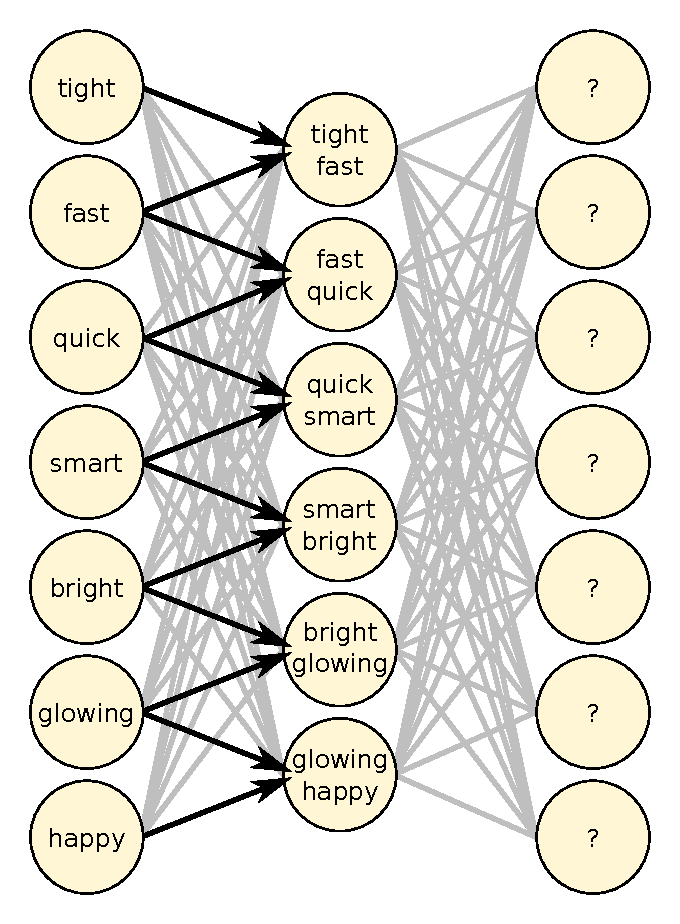
\includegraphics[width=\linewidth]{neural-network-for-language.pdf}

\column{0.6\linewidth}
We made a database of exact words.

\vspace{0.5 cm}
Using a neural network, LLMs encode sequences of meanings, not the exact words (or letters).

\vspace{0.5 cm}
This makes it more sensitive to both synonyms and multi-word context.
\end{columns}
\end{frame}

\begin{frame}{From Andrej Karpathy's {\it Unreasonable Effectiveness of RNNs}}
\Large
\vspace{0.3 cm}
\begin{columns}
\column{0.64\linewidth}
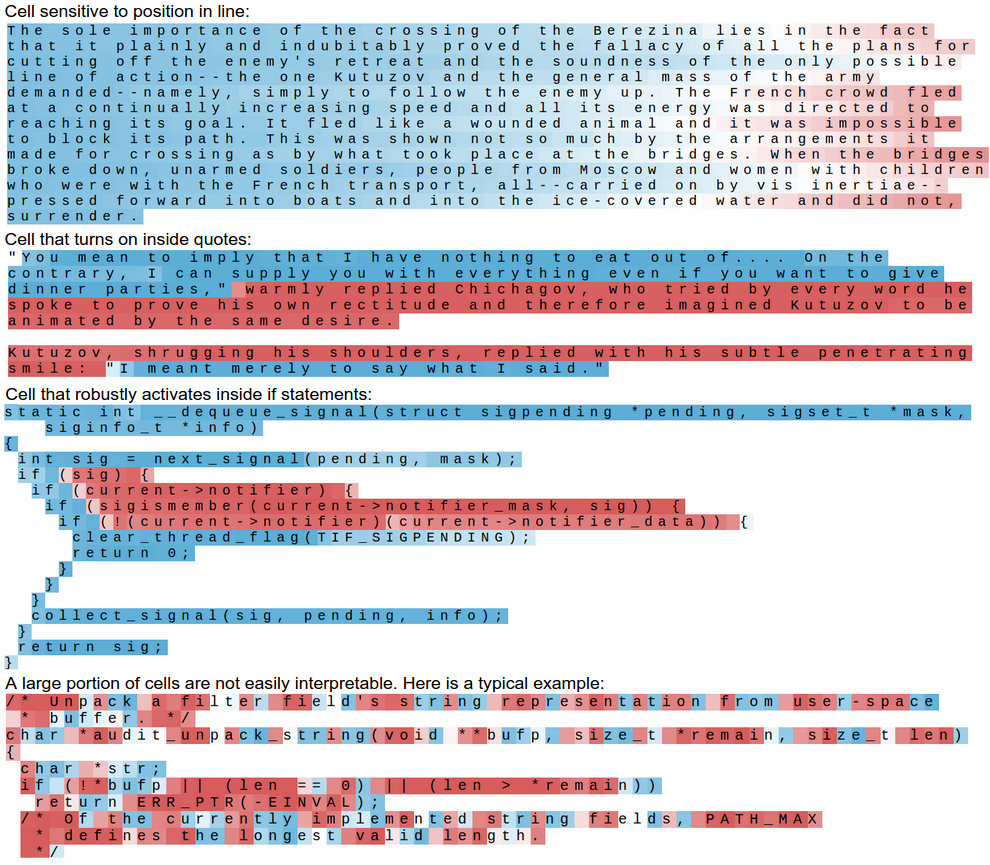
\includegraphics[width=\linewidth]{pane1.png}

\column{0.36\linewidth}
Activation of individual cells in neural networks that generate text.

\vspace{0.5 cm}
\textcolor{blue}{blue} is $+1$, \textcolor{red}{red} is $-1$.

\large
\vspace{0.5 cm}
Some cells are gates that turn on and off submodels with different correlations, but most cells don't act on their own at all.
\end{columns}
\end{frame}

\begin{frame}{$2^{\mbox{nd}}$ difference: attention mechanism (from language translation)}
\Large
\vspace{0.35 cm}
\begin{columns}
\column{1.1\linewidth}
\only<1>{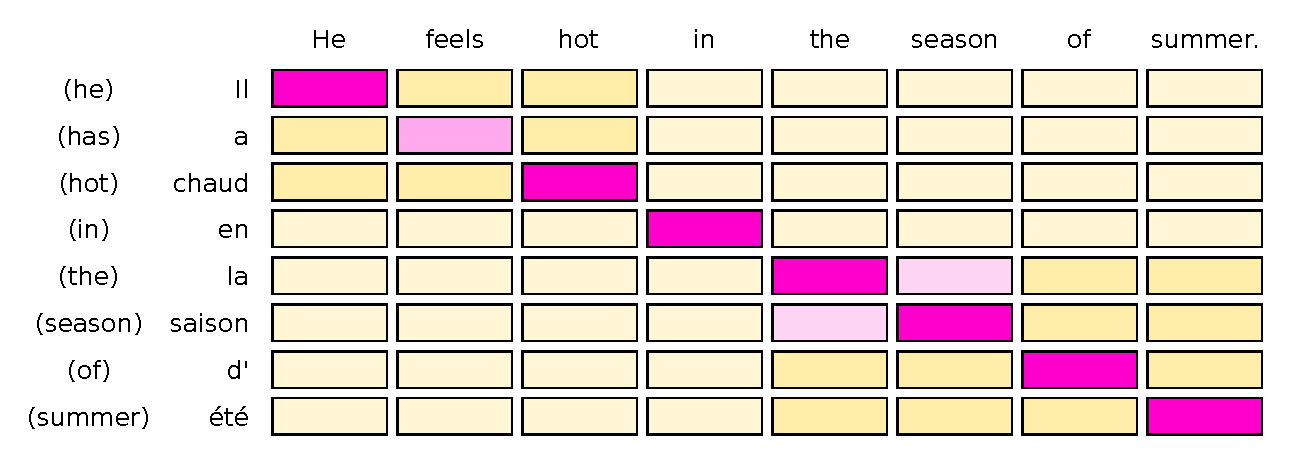
\includegraphics[width=\linewidth]{cross-attention-in-french.pdf}}\only<2>{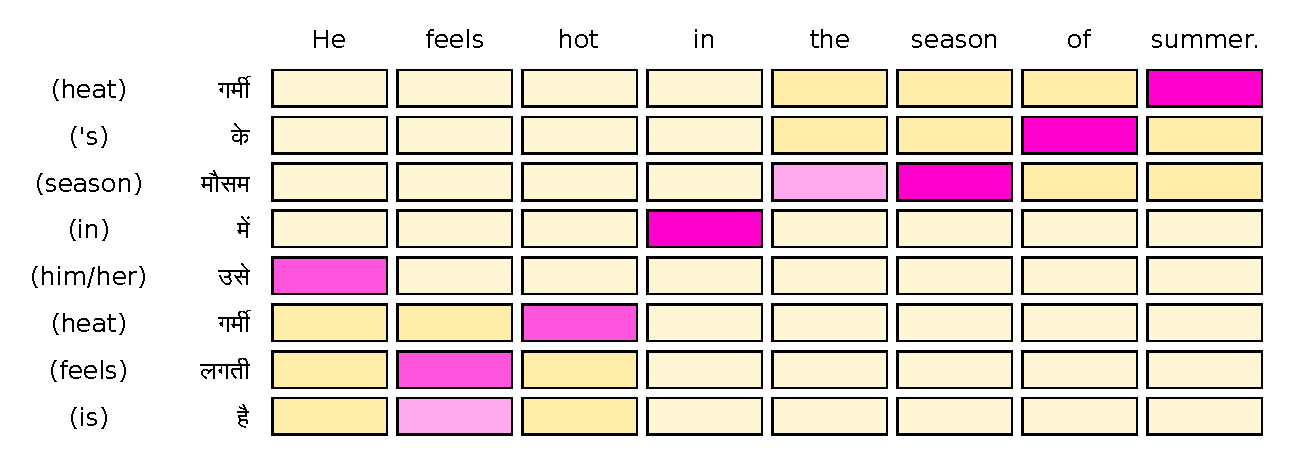
\includegraphics[width=\linewidth]{cross-attention-in-hindi.pdf}}
\end{columns}

\vspace{0.25 cm}
Our context window was exactly 5 tokens long. LLMs train an ``attention'' distribution that varies in size and shape for each token.
\end{frame}

\begin{frame}{From D.\ Bahdanau, K.\ Cho, Y.\ Bengio (2014)}
\Large
\vspace{-0.5 cm}
\begin{columns}
\column{0.58\linewidth}
\hspace{-0.75 cm}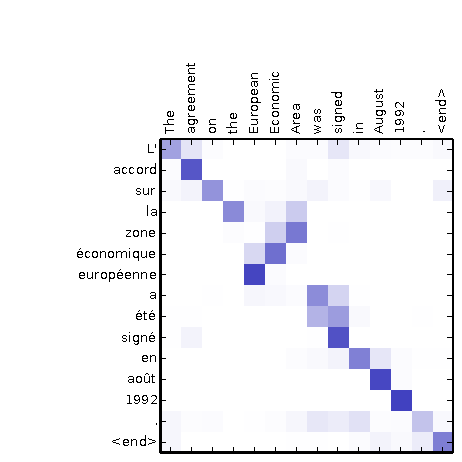
\includegraphics[width=\linewidth]{real-cross-attention-a.pdf}

\column{0.58\linewidth}
\hspace{-1 cm}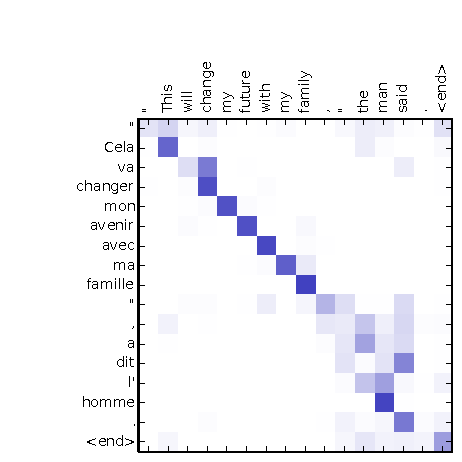
\includegraphics[width=\linewidth]{real-cross-attention-d.pdf}
\end{columns}
\end{frame}

\begin{frame}{$3^{\mbox{rd}}$ difference: LLMs are huge}
\vspace{0.5 cm}
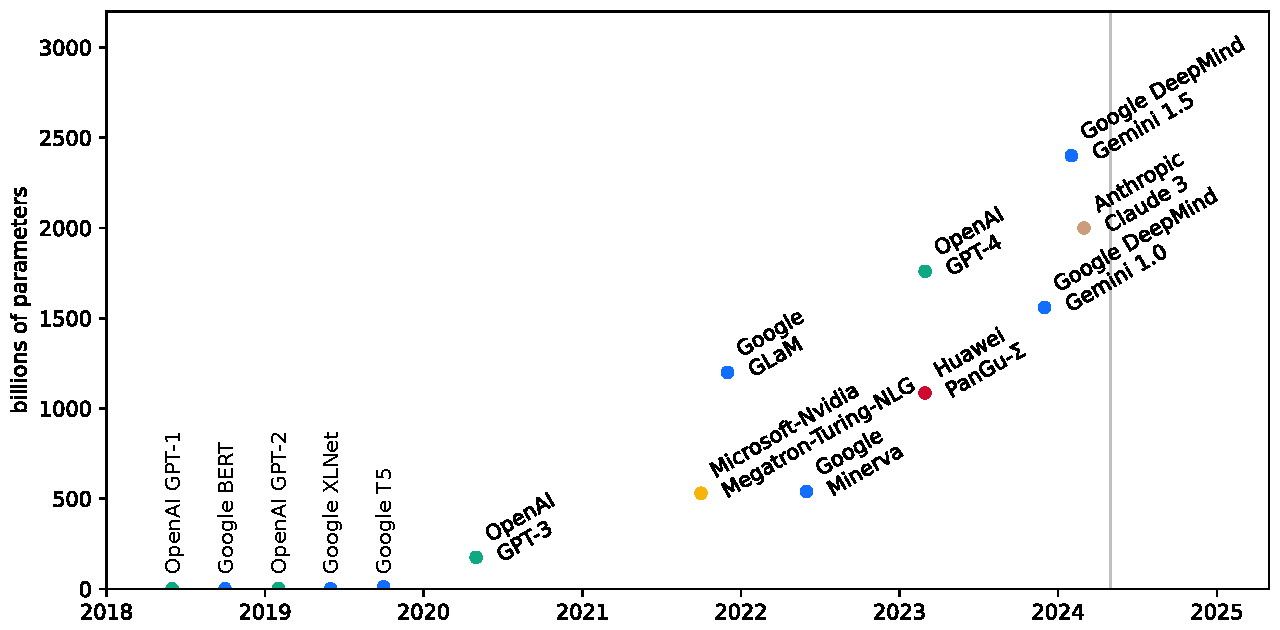
\includegraphics[width=\linewidth]{llm-number-of-parameters.pdf}
\end{frame}

\begin{frame}{$4^{\mbox{th}}$ difference: chat LLMs are fine-tuned for usefulness}
\vspace{0.5 cm}
\begin{columns}
\column{0.92\linewidth}
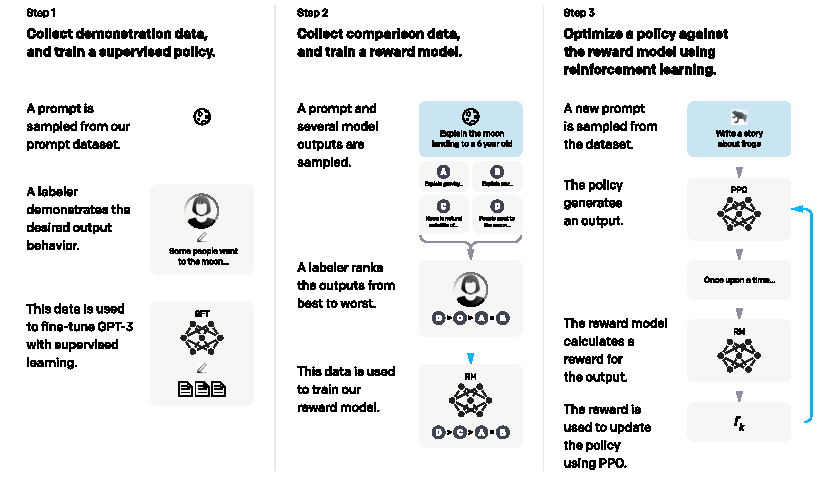
\includegraphics[width=\linewidth]{fine-tuning-for-chat.pdf}
\end{columns}
\end{frame}

\begin{frame}{From L.\ Ouyang et al.\ /OpenAI (2022)}
\large
\vspace{0.4 cm}
\begin{columns}
\column{0.9\linewidth}
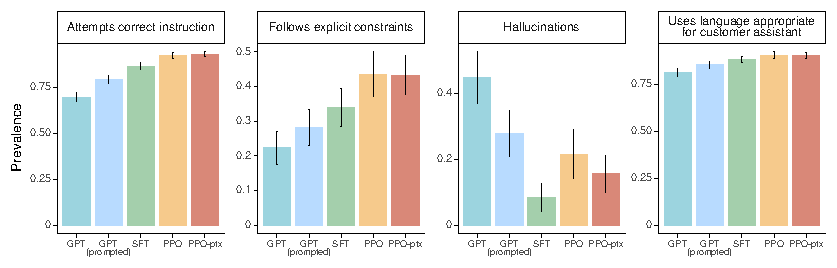
\includegraphics[width=\linewidth]{fine-tuning-for-chat-results.pdf}
\end{columns}

\vspace{0.2 cm}
\begin{columns}
\column{0.68\linewidth}
After the big model (GPT-3) was trained on raw text completions, the neural network weights were re-fitted to optimize for helpfulness, as defined by 40 paid users.

\column{0.25\linewidth}
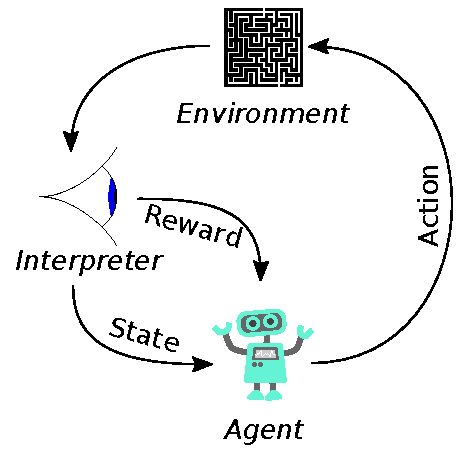
\includegraphics[width=\linewidth]{Reinforcement_learning_diagram.pdf}
\end{columns}
\end{frame}

\end{document}
